
\serie{Sommes de relatifs}

\begin{exercice}
Recopie dans ton cahier, effectue les additions puis relie chaque calcul à son résultat :
\begin{center}
 \begin{tabularx}{0.95\linewidth}{|cc|X|cc|}
  \cline{1-2}\cline{4-5}
  $(-12) + (-4)$ & $\cdot$ & & $\cdot$ & $+4$ \\ \cline{1-2}\cline{4-5}
  $(+12) + (-4)$ & $\cdot$ & & $\cdot$ & $-20$ \\ \cline{1-2}\cline{4-5}
  $(-12) + (-8)$ & $\cdot$ & & $\cdot$ & $-16$ \\ \cline{1-2}\cline{4-5}
  $(-8) + (+12)$ & $\cdot$ & & $\cdot$ & $+12$ \\ \cline{1-2}\cline{4-5}
  $(+8) + (+4)$ & $\cdot$ & & $\cdot$ & $+8$ \\ \cline{1-2}\cline{4-5}
  \end{tabularx}
  \end{center}
\end{exercice}

\begin{exercice}
Effectue les additions suivantes :
\begin{colenumerate}{2}
 \item $(+2) + (+7)=$ \dotfill;
 \vspace{.3em}
 \item $(-4) + (+5)=$ \dotfill;
 \vspace{.3em}
 \item $(-8) + (-14)=$ \dotfill;
  \vspace{.3em}
 \item $(+9) + (-9)=$ \dotfill;
  \vspace{.3em}
 \item $(-20) + (-12)=$ \dotfill;
  \vspace{.3em}
 \item $(+40) + (-60)=$ \dotfill;
  \vspace{.3em}
 \item $(-36) + (+18)=$ \dotfill;
  \vspace{.3em}
 \item $(-25) + (+0)=$\dotfill.
 \end{colenumerate}
\end{exercice}


\begin{exercice}
Effectue les additions suivantes :
\begin{enumerate}
 \item $(-8) + (-16)=$ \dotfill;
   \vspace{.3em}
 \item $(+24) + (-4)=$ \dotfill;
    \vspace{.3em}
 \item $(-14) + (-3)=$ \dotfill;
    \vspace{.3em}
 \item $(-7) + (+7)=$ \dotfill;
    \vspace{.3em}
 \item $(+14) + (+8)=$ \dotfill;
    \vspace{.3em}
 \item $(+11) + (+33)=$ \dotfill;
    \vspace{.3em}
 \item $(+30) + (-47)=$ \dotfill;
    \vspace{.3em}
 \item $(+19) + (+1)=$ \dotfill;
    \vspace{.3em}
 \item $(-11) + (-13)=$ \dotfill;
    \vspace{.3em}
 \item $(+63) + (-63)=$\dotfill.
 \end{enumerate}
\end{exercice}


\begin{exercice}
Effectue les additions suivantes :
\begin{colenumerate}{1}
 \item $(-2,3) + (-4,7)=$ \dotfill ;
    \vspace{.3em}
 \item $(+6,8) + (-9,9)=$ \dotfill;
    \vspace{.3em}
 \item $(-3,5) + (+1,8)=$ \dotfill;
    \vspace{.3em}
 \item $(-2,51) + (-0)=$ \dotfill;
    \vspace{.3em}
 \item $(-7,8) + (-2,1)=$ \dotfill;
    \vspace{.3em}
 \item $(+13,4) + (-20,7)=$ \dotfill;
    \vspace{.3em}
 \item $(-10,8) + (+11,2)=$ \dotfill;
    \vspace{.3em}
 \item $(+17) + (+5,47)=$\dotfill.
 \end{colenumerate}
\end{exercice}


\begin{exercice}[La pyramide]
Recopie puis complète les pyramides suivantes sachant que le nombre contenu dans une case est la somme des nombres contenus dans les deux cases situées en dessous de lui : \\

\begin{minipage}[c]{0.48\linewidth}
\begin{center} 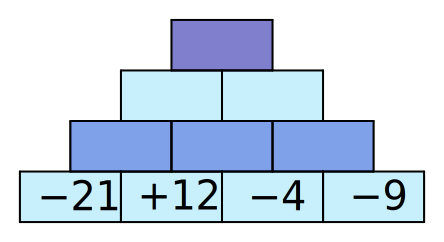
\includegraphics[width=4cm]{pyramide1_OpererRelatifs} \end{center}
\end{minipage} \hfill%
 \begin{minipage}[c]{0.48\linewidth}
\begin{center} 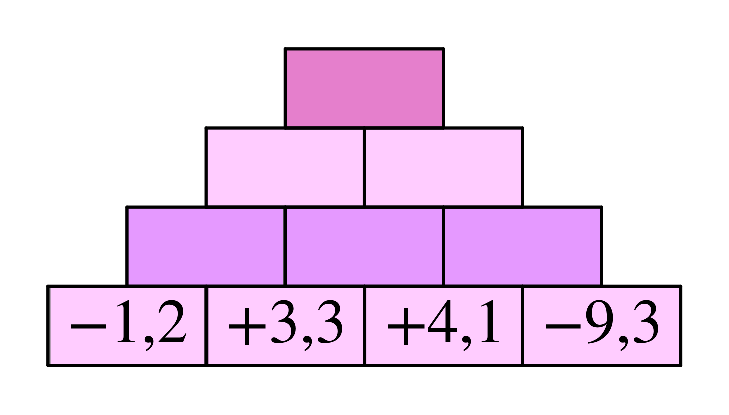
\includegraphics[width=4cm]{pyramide2_OpererRelatifs} \end{center} 
\end{minipage} \\
\end{exercice}


\begin{exercice}[La pyramide (bis)]
\vspace{0.5em}
\begin{minipage}[c]{0.48\linewidth}
\begin{center} 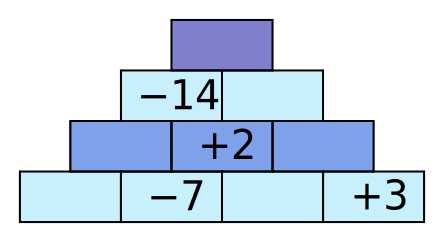
\includegraphics[width=3.8cm]{pyramide3_OpererRelatifs} \end{center}
 \end{minipage} \hfill%
 \begin{minipage}[c]{0.48\linewidth}
\begin{center} 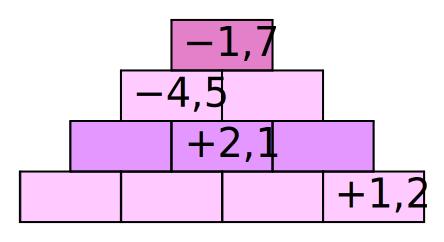
\includegraphics[width=3.8cm]{pyramide4_OpererRelatifs} \end{center}
  \end{minipage} \\
\end{exercice}


\begin{exercice}
Effectue les additions suivantes en détail :
\begin{enumerate}
 \item $(+3) + (-7) + (-8) + (+2)$ ;
 \item $(-9) + (-14) + (+25) + (-3)$ ;
 \item $(-2,3) + (-12,7) + (+24,7) + (-1,01)$ ;
 \item $(+7,8) + (+2,35) + (-9,55) + (+4)$.
 \end{enumerate}
\end{exercice}


\begin{exercice}
Calcule les sommes suivantes en détail :
\begin{enumerate}
 \item $(+17) + (-5) + (+4) + (+5) + (-3)$ ;
 \item $(-12) + (-4) + (+7) + (+8) + (-6)$ ;
 \item $(-3) + (+5) + (-4) + (+6) + (-1)$ ;
 \item $(+1,2) + (-4,2) + (+7,1) + (-6,7)$.
 \end{enumerate}
\end{exercice}


\begin{exercice}[Durées de vie]
Remarque : pour cet exercice, n'oubliez pas que l'an 0 n'existe pas.
\begin{enumerate}
 \item Cicéron est né en l'an $-23$ et est mort en l'an 38. Combien de temps a-t-il vécu ?
 \item Thalès de Milet est né en l'an $-625$ et est mort à l'âge de 78 ans. En quelle année est-il mort ?
 \item L'Empire de Césarius a été créé en $-330$ et s'est terminé en 213. Combien de temps a-t-il duré ?
 \item Ératosthène est mort en l'an $-194$ à l'âge de 82 ans. En quelle année est-il né ?
 \item Thésée avait 11 ans à la mort de Claudius. Claudius est mort en l'an $-18$. Thésée est mort en l'an 31. À quel âge est mort Thésée ?
 \end{enumerate}
\end{exercice}

%%%%%%%%%%%%%%%%%%%%%%%%%%%%%%%%%%%%%%%%%%%%%%%%%%%%%%%%%%%%%%%%%%%

%%%%%%%%%%%%%%%%%%%%%%%%%%%%%%%%%%%
%MiseEnPage
%%%%%%%%%%%%%%%%%%%%%%%%%%%%%%%%%%%
\newpage
%%%%%%%%%%%%%%%%%%%%%%%%%%%%%%%%%%%

\serie{Différences de relatifs}

\begin{exercice}
Complète afin de transformer les soustractions suivantes en additions :
\begin{enumerate}
 \item $(+2) - (+7) = (+2) + (\ldots \ldots)$ ;
 \item $(-4) - (+5) = (-4) + (\ldots \ldots)$ ;
 \item $(-8) - (-14) =  (\ldots \ldots) + (\ldots \ldots)$ ;
 \item $(+9) - (-9) =  (\ldots \ldots) + (\ldots \ldots)$.
 \end{enumerate}
\end{exercice}

\begin{exercice}
Transforme les soustractions suivantes en additions puis effectue-les :
\begin{colenumerate}{1}
 \item $(+4) - (+15)$ \dotfill;
 \vspace{0.4em}
 \item $(-12) - (+5)$ \dotfill;
 \vspace{0.4em}
 \item $(-10) - (-7)$ \dotfill;
 \vspace{0.4em}
 \item $(+14) - (-4)$ \dotfill;
 \vspace{0.4em}
 \item $(+6) - (+6)$ \dotfill;
 \vspace{0.4em}
 \item $(-20) - (+7)$\dotfill.
 \end{colenumerate}
\end{exercice}


\begin{exercice}
Effectue les soustractions suivantes :
\begin{colenumerate}{1}
 \item $(-2,6) - (+7,8)$ \dotfill;
 \vspace{0.4em}
 \item $(+6,4) - (+23,4)$ \dotfill;
 \vspace{0.4em}
 \item $(+4,5) - (-12,8)$ \dotfill;
 \vspace{0.4em}
 \item $(-2,7) - (-9,9)$ \dotfill;
 \vspace{0.4em}
 \item $(-12,8) - (+9,5)$ \dotfill;
 \vspace{0.4em}
 \item $(+6,7) - (+2,4)$ \dotfill;
 \vspace{0.4em}
 \item $(+8,1) - (-13,6)$ \dotfill;
 \vspace{0.4em}
 \item $(-12,7) - (-9,8)$\dotfill.
 \end{colenumerate}
\end{exercice}


\begin{exercice}
Pour chaque expression, transforme les soustractions en additions puis effectue les calculs :
\begin{enumerate}
 \item $(+4) - (-2) + (-8) - (+7)$ ;
 \item $(-27) - (-35) - (-20) + (+17)$ ;
 \item $(+3,1) + (-3,5) - (+7,8) - (+1,6)$ ;
 \item $(-16,1) - (+4,25) + (+7,85) - (+1,66)$.
 \end{enumerate}
\end{exercice}


\begin{exercice}
Jean et Saïd vont à la fête foraine. Ils misent la même somme d'argent au départ. Jean perd 2,30 CHF puis gagne 7,10 CHF. Saïd gagne 6 CHF puis perd 1,30 CHF. Lequel des deux amis a remporté le plus d'argent à la fin du jeu ?
\end{exercice}

%%%%%%%%%%%%%%%%%%%%%%%%%%%%%%%%%%%
%MiseEnPage
%%%%%%%%%%%%%%%%%%%%%%%%%%%%%%%%%%%
\columnbreak
%%%%%%%%%%%%%%%%%%%%%%%%%%%%%%%%%%%


\begin{exercice}
Pour chaque expression, transforme les soustractions en additions puis calcule les sommes :
\begin{enumerate}
 \item $(+12) - (-6) + (-2) + (+7) - (+8)$ ;
 \item $(-20) - (+14) + (+40) + (-12) - (-10)$ ;
 \item $(-2,4) + (-7,1) - (-3,2) - (+1,5) + (+8,4)$ ;
 \item $(+1,9) - (-6,8) + (-10,4) + (+7,7) - (+2)$.
 \end{enumerate}
\end{exercice}


\begin{exercice}
Le professeur Sésamatheux donne à ses élèves un questionnaire à choix multiples (Q.C.M) comportant huit questions. Il note de la façon suivante :
\begin{itemize}
 \item Réponse fausse ($F$) : $-3$
 \item Sans réponse ($S$) : $-1$
 \item Réponse bonne ($B$) : $+4$
 \end{itemize}
 \vspace{-0.4em}
 \begin{enumerate}
 \item Calcule la note de Wenda dont les résultats aux questions sont : $F$ ; $B$ ; $S$ ; $F$ ; $F$ ; $B$ ; $B$ ; $S$. 
 \item Quelle est la note la plus basse qu'un élève peut obtenir ? Et la plus haute ?
 \item Quels sont les résultats possibles pour Emeline qui a obtenu une note $+4$ ?
 \end{enumerate}
\end{exercice}


\begin{exercice}
Calcule astucieusement les expressions suivantes :
\begin{enumerate}
 \item $(+14) + (-45) + (-14) + (+15)$ ;
 \item $(-1,4) + (-1,2) + (+1,6) - (+1,6)$ ;
 \item $(+1,35) + (-2,7) - (-0,65) + (-1,3)$ ;
 \item $(-5,45) - (-0,45) + (+1,3) - (-1) - (+1,3)$.
 \end{enumerate}
\end{exercice}


\begin{exercice}
Remplace les pointillés par le nombre qui convient :
\begin{enumerate}
 \item $(-10) - \ldots \ldots  = 25$ ;
 \item $(+16) - \ldots \ldots  = 42$ ;
 \item $(+25) - (-13) + (-5) + \ldots \ldots = 26$ ;
 \item $(-63) + (-8) - \ldots \ldots + (+18) = 21$.
 \end{enumerate}
\end{exercice}


\begin{exercice}
Pour chaque cas, calcule en détail $x + y - z$ et $x - (y + z)$ :
\begin{center}
\begin{tabularx}{0.4\linewidth}{|X|c|c|c|}
\hline
 & x & y & z \\ \hline
\textbf{a.} & 10 & $-3$ & 8 \\ \hline
\textbf{b.} & $-6$ & $-5$ & 2 \\ \hline
\textbf{c.} & 3 & $-8$ & $-2$ \\ \hline
\textbf{d.} & 7 & $-2$ & $-5$ \\ \hline
 \end{tabularx}
 \end{center}
\end{exercice}

%%%%%%%%%%%%%%%%%%%%%%%%%%%%%%%%%%%%%%%%%%%%%%%%%%%%%%%%%%%%%%%%%%%
%%%%%%%%%%%%%%%%%%%%%%%%%%%%%%%%%%%
%MiseEnPage
%%%%%%%%%%%%%%%%%%%%%%%%%%%%%%%%%%%
\newpage
%%%%%%%%%%%%%%%%%%%%%%%%%%%%%%%%%%%


\serie{Écriture simplifiée}

\begin{exercice}
Relie chaque expression à son écriture simplifiée :
\begin{center}
 \begin{tabularx}{0.8\linewidth}{|cc|X|cc|}
  \cline{1-2}\cline{4-5}
  $(-8) + (-16)$ & $\bullet$ & & $\bullet$ & $-14 - 3$ \\ \cline{1-2}\cline{4-5}
  $(+24) - (-4)$ & $\bullet$ & & $\bullet$ & $-8 - 16$ \\ \cline{1-2}\cline{4-5}
  $(-14) + (-3)$ & $\bullet$ & & $\bullet$ & $14 + 8$ \\ \cline{1-2}\cline{4-5}
  $(-7) - (+7)$ & $\bullet$ & & $\bullet$ & $-7 - 7$ \\ \cline{1-2}\cline{4-5}
  $(+14) + (+8)$ & $\bullet$ & & $\bullet$ & $24 + 4$ \\ \cline{1-2}\cline{4-5}
  \end{tabularx}
  \end{center}
\end{exercice}


\begin{exercice}
Recopie et complète le tableau :
\begin{center}
\begin{tabularx}{0.98\linewidth}{|c|X|c|}

\hline
 & Écriture avec & Écriture simplifiée \\ 
  & parenthèses &  \\ \hline

\textbf{a.} & \footnotesize{$(-9) - (+13) + (-15)$} & \\ \hline
\textbf{b.} & \footnotesize{$(-10) + (+7) - (-3) - (-3)$} & \\ \hline
\textbf{c.} & \footnotesize{$(+5) - (-2) + (+3) - (+2)$} & \\ \hline
\textbf{d.} & & \footnotesize{$-6 - 8 + 5 - 3$} \\ \hline
\textbf{e.} & & \footnotesize{$15 - 13 - 8 - 7$} \\ \hline
\textbf{f.} & & \footnotesize{$-13 - 5 - 9 + 1$} \\ \hline
 \end{tabularx}
 \end{center}
\end{exercice}


\begin{exercice}
Donne une écriture simplifiée des expressions suivantes en supprimant les parenthèses et les signes qui ne sont pas nécessaires:
\begin{enumerate}
 \item $(-5) + (-3)$ ;
 \item $(-4) - (+6)$ ;
 \item $(+9) - (-3)$ ;
 \item $(+4) + (+7)$ ;
  \item $(+17) - (-5) + (+4) - (+5) - (-3)$ ;
  \item $(-15) + (+3,5) - (-7,9) + (-13,6)$.
  \end{enumerate}
\end{exercice}


\begin{exercice}
Effectue les calculs suivants :
\begin{colenumerate}{2}
 \item $5 - 14$ ;
 \item $8 - 13$ ;
 \item $-6 - 6$ ;
 \item $-13 + 9$ ;
 \item $-53 - 48$ ;
 \item $-2,8 - 4,7$ ;
 \item $-5,7 + 4,4$ ;
 \item $3,2 - 8,9$.
 \end{colenumerate}
\end{exercice}


\begin{exercice}
Effectue en détail :
\begin{colenumerate}{2}
 \item $24 - 36 + 18$ ;
 \item $-13 - 28 + 35$ ;
 \item $-3,8 - 4,4 + 8,2$ ;
 \item $18 - 8 + 4 - 14$ ;
 \item $-1,3 + 4,4 - 21$ ;
 \item $14 - 23 + 56 - 33$.
 \end{colenumerate}
\end{exercice}


\begin{exercice}
Effectue en détail :
\begin{enumerate}
 \item $5 + 13 - 4 + 3 - 6$ ;
 \item $-7 + 5 - 4 - 8 + 13$ ;
 \item $3,5 - 4,2 + 6,5 - 3,5 + 5$ ;
 \item $25,2 + 12 - 4,8 + 24 - 3,4$.
 \end{enumerate}
\end{exercice}


\begin{exercice}
Regroupe les termes astucieusement puis effectue en détail :
\begin{enumerate}
 \item $13 + 15 + 7 - 15$ ;
 \item $-8 + 4 + 18 - 2 + 12 + 6$ ;
 \item $4,3 - 7,4 + 4 - 2,25 + 6,7 + 3,4 - 2,75$ ;
 \item $-2,5 + 4,8 - 3,6 + 0,2 + 2,5$.
 \end{enumerate}
\end{exercice}


\begin{exercice}
Calcule les expressions suivantes, en détail :
\begin{enumerate}
 \item $(-3 + 9) - (4 - 11) - (-5 - 6)$ ;
 \item $-3 + 12 - (13 - 8) - (3 + 8)$ ;
 \item $-3 - [4 - (3 - 9)]$.
 \end{enumerate}
\end{exercice}


\begin{exercice}[Températures]
Pour mesurer la température, il existe plusieurs unités. Celle que nous utilisons en Suisse est le degré Celsius ($^{\circ}$C). Cette unité est faite de façon à ce que la température à laquelle l'eau se transforme en glace est $0^{\circ}$C et celle à laquelle l'eau se transforme en vapeur est $100^{\circ}$C. Dans cette échelle, il existe des températures négatives. \\[0.5em]
Il existe une autre unité, le Kelvin (K), dans laquelle les températures négatives n'existent pas. Pour passer de l'une à l'autre, on utilise la formule :
\begin{center} $T_\text{Kelvin} = T_\text{degrés Celsius} + 273,15$ \end{center}
Ainsi, $10^{\circ}$C correspondent à 283,15 K.
\begin{enumerate}
 \item Convertis en Kelvin les températures suivantes : $24^{\circ}$C ; $-3^{\circ}$C et $-22,7^{\circ}$C ;
 \item Convertis en degré Celsius les températures suivantes : 127,7 K ; 276,83 K ; 204 K et 500 K ;
 \item Quelle est en Kelvin la plus petite température possible ? À quelle température en degré Celsius correspond-elle ? Cette température est appelée le zéro absolu.
 \end{enumerate}
\end{exercice}
